\section{Results}
Results for two different cases are being presented, one the one-dimensional Ising Model and another for the the two-dimensional Ising model. We begin with looking at the. 1D Ising model.

\subsection{1D Ising model}
\subsubsection{Fitting with linear regression}
For linear regression we got coefficients of $\bm{J}$ in \eqref{eq:1d-ising-linreg} as the following,
\begin{figure}
    \centering
    \begin{subfigure}[b]{0.5\textwidth}
        \centering
        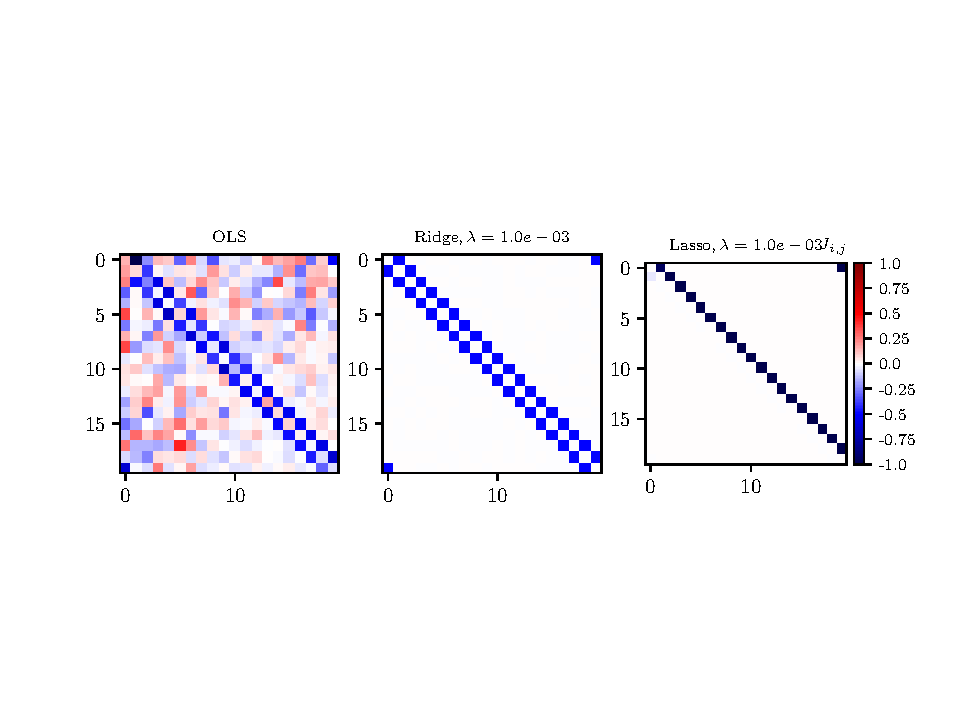
\includegraphics[scale=0.5]{../fig/regression_ising_1d_heatmap_lambda0.001.pdf}
        \caption{$\lambda=10^{-3}$}
        \label{fig:linreg-hm-1e-3}
    \end{subfigure} \\
    \begin{subfigure}[b]{0.5\textwidth}
        \centering
        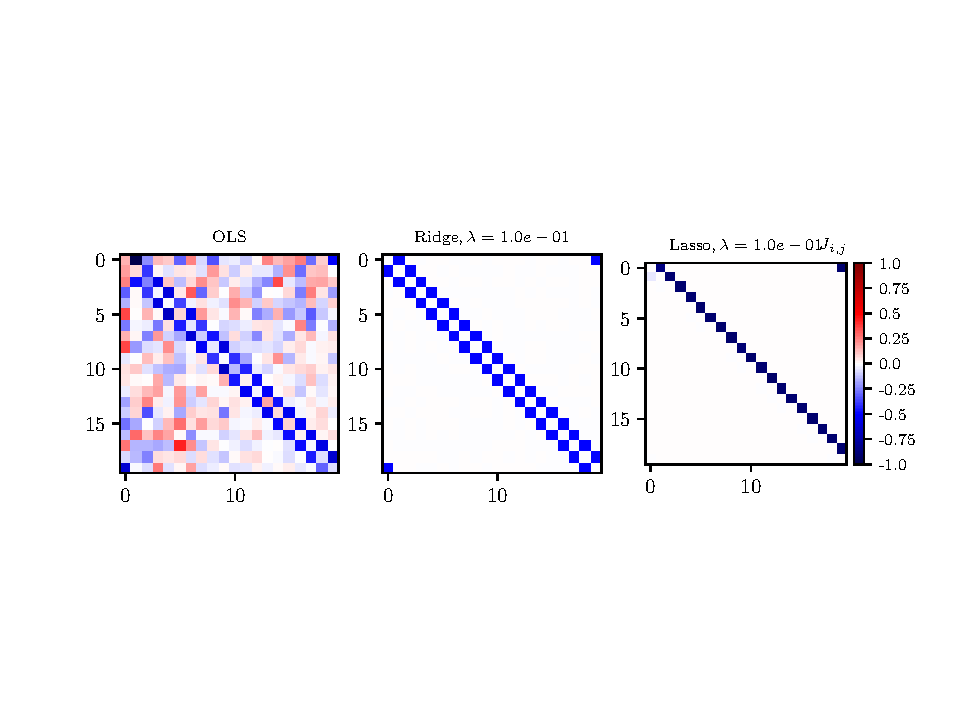
\includegraphics[scale=0.5]{../fig/regression_ising_1d_heatmap_lambda0.1.pdf}
        \caption{$\lambda=10^{-1}$}
        \label{fig:linreg-hm-1e-1}
    \end{subfigure} \\
    \begin{subfigure}[b]{0.5\textwidth}
        \centering
        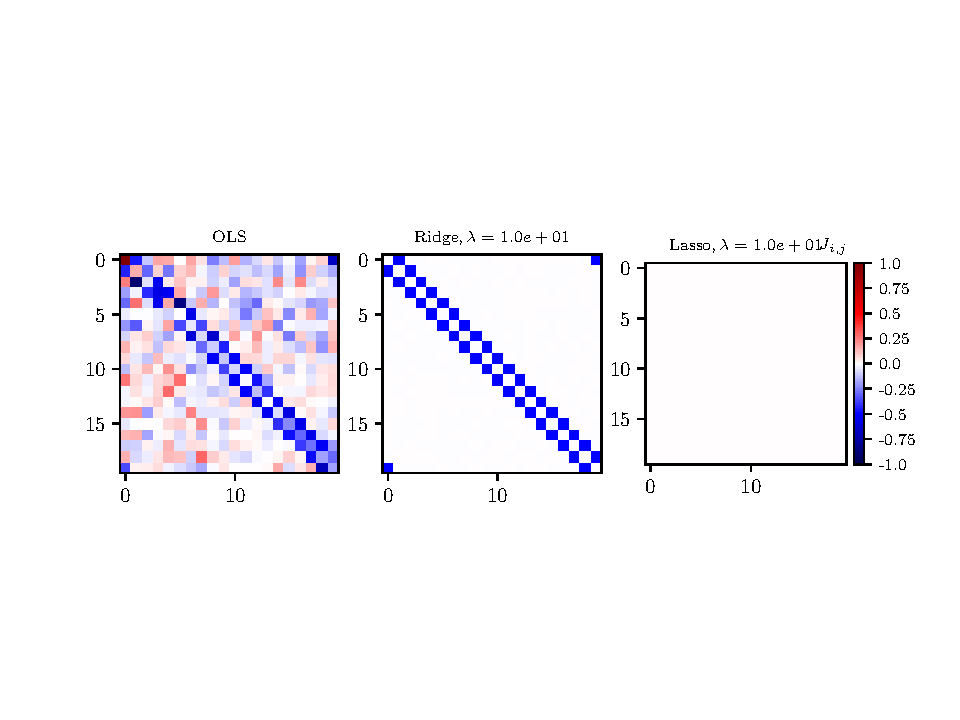
\includegraphics[scale=0.5]{../fig/regression_ising_1d_heatmap_lambda10.0.pdf}
    \caption{$\lambda=10^{1}$}
        \label{fig:linreg-hm-1e2}
    \end{subfigure}
    \caption{Heat map plots of the $\bm{J}$ in \eqref{eq:1d-ising-linreg} retrieved from OLS, Ridge and Lasso. Gathered using $N_\mathrm{train}=5000$.}
    \label{fig:bias-var-franke}
\end{figure}

The $R^2$ score of the OLS, Ridge and Lasso can be seen in figure \ref{fig:linreg-r2},
\begin{figure}[H]
    \centering
    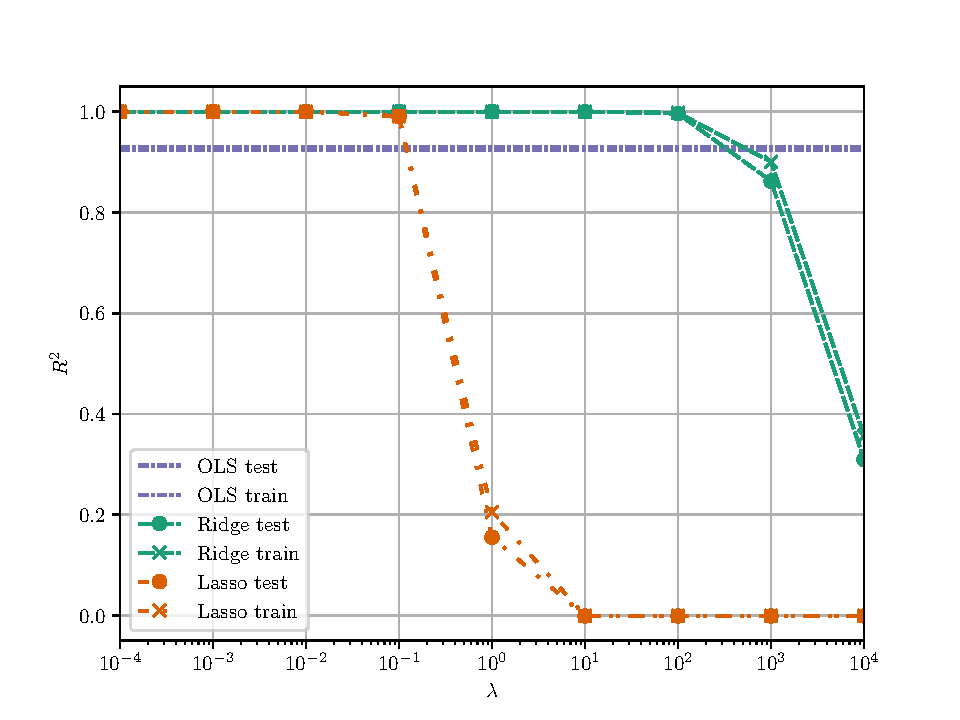
\includegraphics[scale=1.0]{../fig/r2_ols_ridge_lasso.pdf}
    \caption{$R^2$ score for different Ordinary Least Squares(OLS), Ridge and Lasso regression. Retrieved $N_\mathrm{train}=5000$ on a 1D Ising model of size $L=20$.
    \label{fig:linreg-r2}
\end{figure}

The bias-variance decomposition for Ridge and Lasso using bootstrap and cross validation can be viewed in figure \ref{fig:linreg-bias-variance-decomp-ridge} and \ref{fig:linreg-bias-variance-decomp-lasso}.

\begin{figure}[H]
    \centering
    \begin{subfigure}[b]{0.5\textwidth}
        \centering
        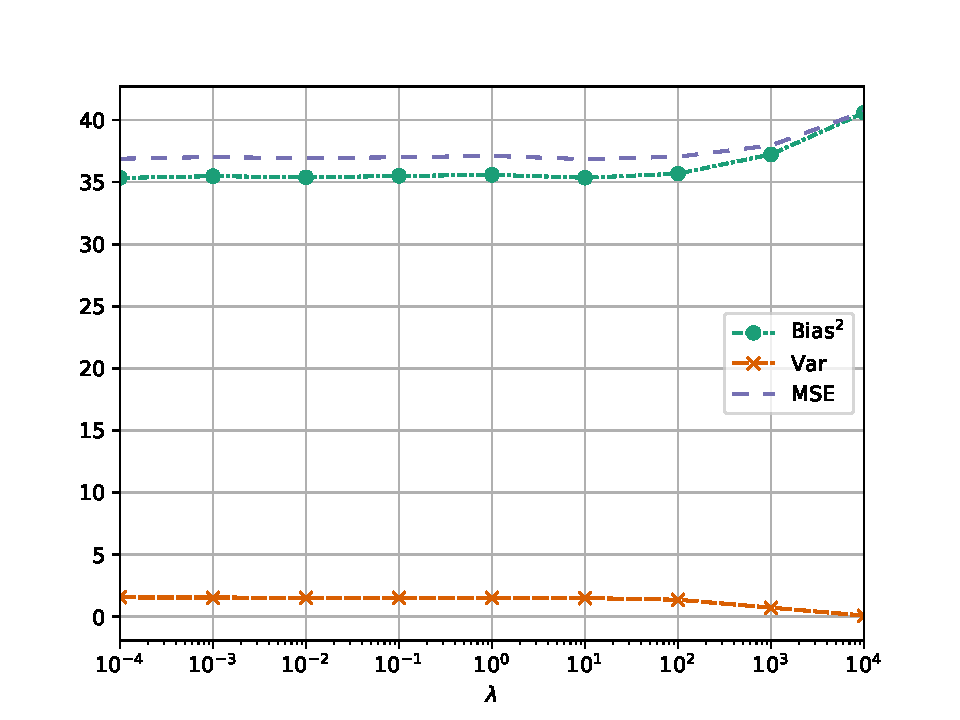
\includegraphics[scale=0.5]{../fig/ridge_bs_bias_variance_analysis.pdf}
        \caption{Bootstrap.}
        \label{fig:linreg-bias-variance-decomp-bs-ridge}
    \end{subfigure}%
    \begin{subfigure}[b]{0.5\textwidth}
        \centering
        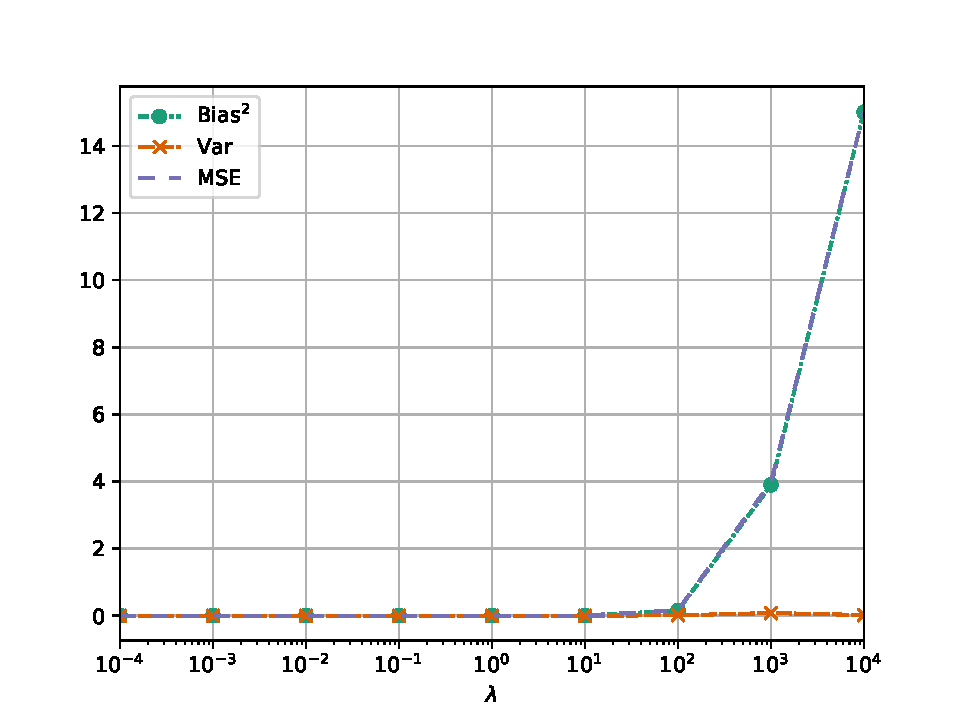
\includegraphics[scale=0.5]{../fig/ridge_cv_bias_variance_analysis.pdf}
        \caption{$k$-fold Cross Validation.}
        \label{fig:linreg-bias-variance-decomp-cv-ridge}
    \end{subfigure}
    \caption{A bias-variance decomposition of Ridge regression using bootstrapping\ref{fig:linreg-bias-variance-decomp-bs-ridge} and cross-validation\ref{fig:linreg-bias-variance-decomp-cv-ridge}.}
    \label{fig:linreg-bias-variance-decomp-ridge}
\end{figure}

\begin{figure}[H]
    \centering
    \begin{subfigure}[b]{0.5\textwidth}
        \centering
        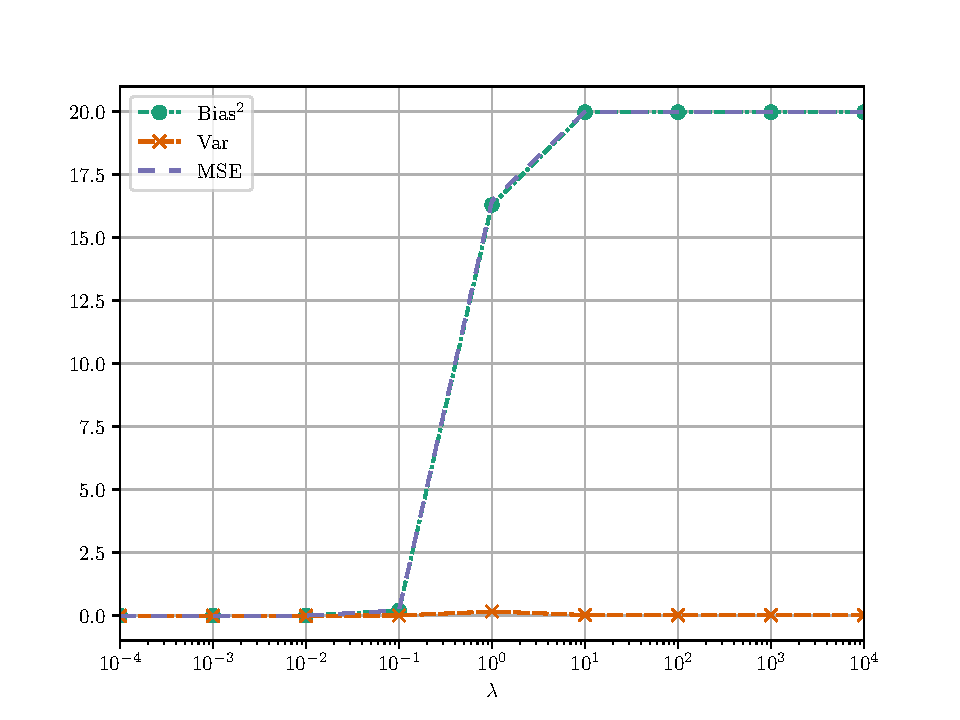
\includegraphics[scale=0.5]{../fig/lasso_bs_bias_variance_analysis.pdf}
        \caption{Bootstrap.}
        \label{fig:linreg-bias-variance-decomp-bs-lasso}
    \end{subfigure}%
    \begin{subfigure}[b]{0.5\textwidth}
        \centering
        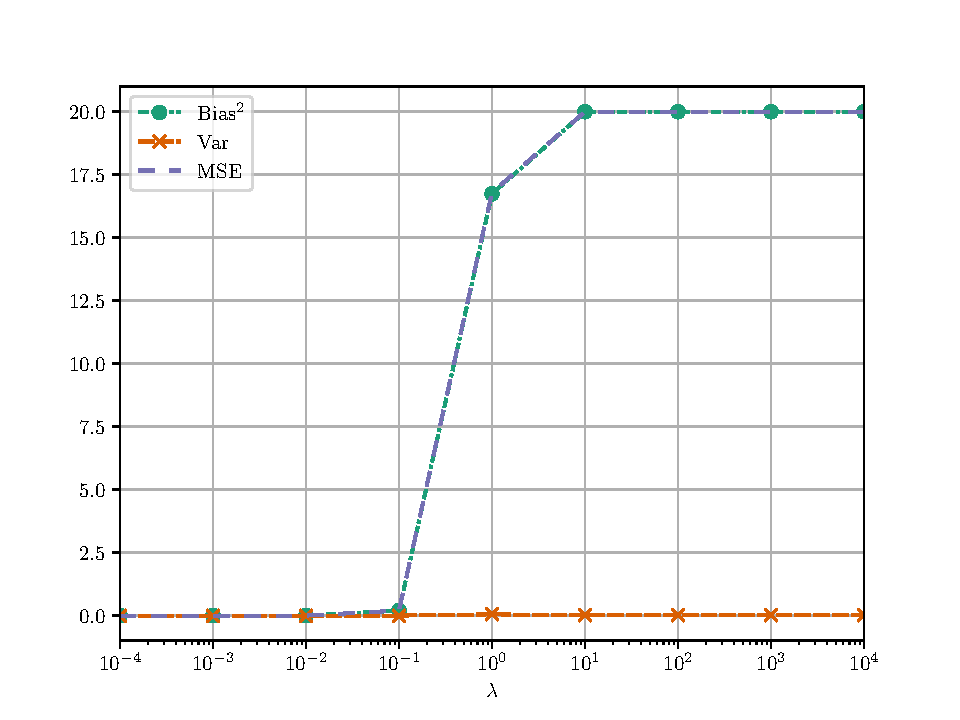
\includegraphics[scale=0.5]{../fig/lasso_cv_bias_variance_analysis.pdf}
        \caption{$k$-fold Cross Validation.}
        \label{fig:linreg-bias-variance-decomp-cv-lasso}
    \end{subfigure}
    \caption{A bias-variance decomposition of Lasso regression using bootstrapping\ref{fig:linreg-bias-variance-decomp-bs-lasso} and cross-validation\ref{fig:linreg-bias-variance-decomp-cv-lasso}.}
    \label{fig:linreg-bias-variance-decomp-lasso}
\end{figure}

\subsubsection{Fitting with a neural network}
By setting the output activation function to the identity and by having zero hidden layers, we are essentially performing a regression analysis on the 1D Ising model. We generate the same amount of data by inputing the same RNG(random number generator) seed. A fit using $N_\mathrm{train}=400$ and $N_\mathrm{train}=5000$ can be seen in respectively figure 

\begin{figure}[H]
    \centering
    \begin{subfigure}[b]{0.5\textwidth}
        \centering
        \includegraphics[scale=0.5]{../fig/}
        \caption{$N_\mathrm{train}=400$}
        \label{fig:mlp-reg-heatmap400}
    \end{subfigure}%
    \begin{subfigure}[b]{0.5\textwidth}
        \centering
        \includegraphics[scale=0.5]{../fig/}
        \caption{$N_\mathrm{train}=5000$}
        \label{fig:mlp-reg-heatmap5000}
    \end{subfigure}
    \caption{Heat map plot of the coefficients of $\bm{J}$ in \eqref{eq:1d-ising-linreg} using neural networks with different regularizations.}
    \label{fig:mlp-coefs}
\end{figure}

The $R^2$ score of the neural network using L$^1$, L$^2$ and no regularization can be seen in figure \ref{fig:mlp-r2},
\begin{figure}[H]
    \centering
    \begin{subfigure}[b]{0.5\textwidth}
        \centering
        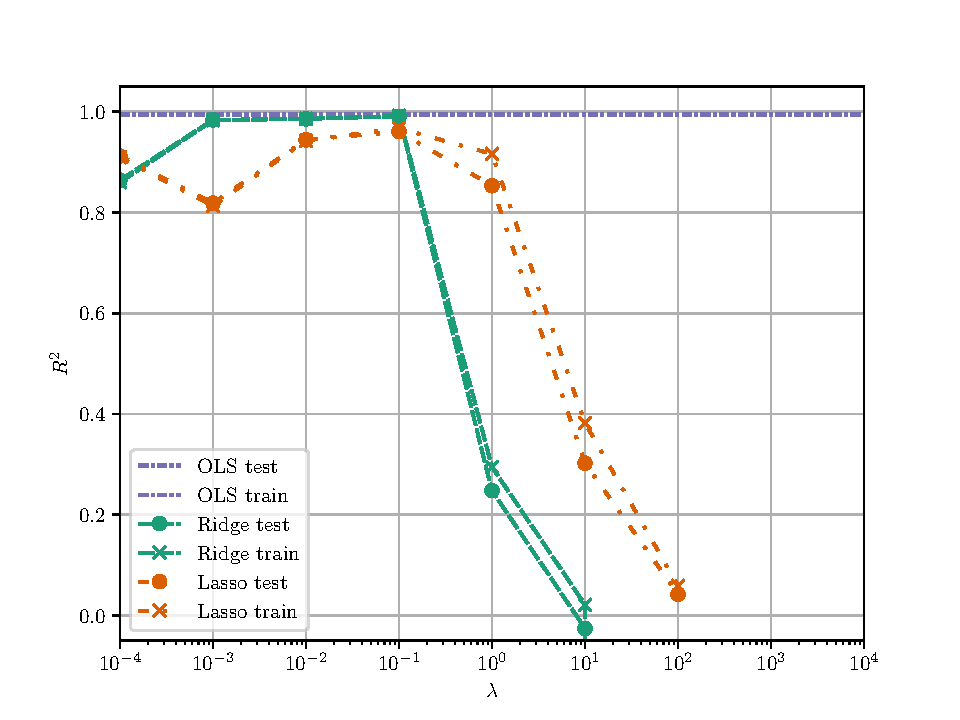
\includegraphics[scale=0.5]{../fig/mlp_r2_ols_ridge_lasso800.pdf}
        \caption{$N_\mathrm{train}=400$}
        \label{fig:mlp-r2-800}
    \end{subfigure}%
    \begin{subfigure}[b]{0.5\textwidth}
        \centering
        \includegraphics[scale=0.5]{../fig/mlp_r2_ols_ridge_lasso10000.pdf}
        \caption{$N_\mathrm{train}=5000$}
        \label{fig:mlp-r2-5000}
    \end{subfigure}
    \caption{$R^2$ score for the neural network using L$^1$, L$^2$ and no regularization. Retrieved $N_\mathrm{train}=400$ on the left and $N_\mathrm{train}=5000$ on the right, for a 1D Ising model of size $L=20$.
    \label{fig:mlp-r2}
\end{figure}


\subsection{2D Ising model}